\section{Experiments}

We are going to present results on test time performance of approximation with monochromatic filters, and bi-clustering. Moreover,
we additionally support our approximations with visualizations. Major contribution is in lowered evaluation time, while kept prediction performance.
Table \ref{evaluation_time} gives us reference on prediction time for network without approximations.

\begin{table}[t]
\tiny
\parbox{.99\linewidth}{
\centering
\begin{tabular}{rrrrr}
\hline
& Evaluation & & Evaluation &  \\
Layer & Time & Fraction & Time & Fraction \\
& (bs = 1) & (bs = 1) & (bs = 128) & (bs = 128) \\
\hline
Conv1 & & & & \\
MaxPool & & & & \\
LRNormal & & & & \\
Conv2 & & & & \\
MaxPool & & & & \\
LRNormal & & & & \\
Conv3 & & & & \\
MaxPool & & & & \\
Conv4 & & & & \\
Conv5 & & & & \\
MaxPool & & & & \\
FC & & & & \\
FC & & & & \\
FC & & & & \\
Softmax & & & & \\
\hline 
Total & & & & \\
\hline
\end{tabular}
\vspace{5mm}
}
\caption{Evaluation time (in ms) per layer on CPU for (top) AlexNet, (bottom) MattNet. We consider real time application setting (batch size aka bs of 1), and
mass scale annotation (batch size of 128). Results averaged over 8 trials.}
\label{evaluation_time}
\end{table}



\subsection{Monochromatic Filters}
Monochromatic approximation can work well only if color components span few one dimensional subspaces. 
Figure \ref{components}, \ref{components} show that it is indeed case for both AlexNet, as
well as MattNet. In case of AlexNet, we colored with a different colors every feature map, so one dimensional structure
is clearly depicted. For MattNet, we found further low-dimensional structure. All the colors seems to lay close
to two planes. Visualization gives different color to color components laying on every plane. Moreover,
colors span one dimensional subspaces within planes. We further confirmed that monochromatic approximations
are faithful. 

Figures \ref{denoising} and \ref{denoising} shows first layer filters after approximating them 
with monochromatic filters. This corresponds to the projection on one out of ''number of clusters`` 1-dim plane (line).
One can notice that often approximated filters look cleaner than original one.


\begin{figure}[t]
\mbox{
  \subfigure{
      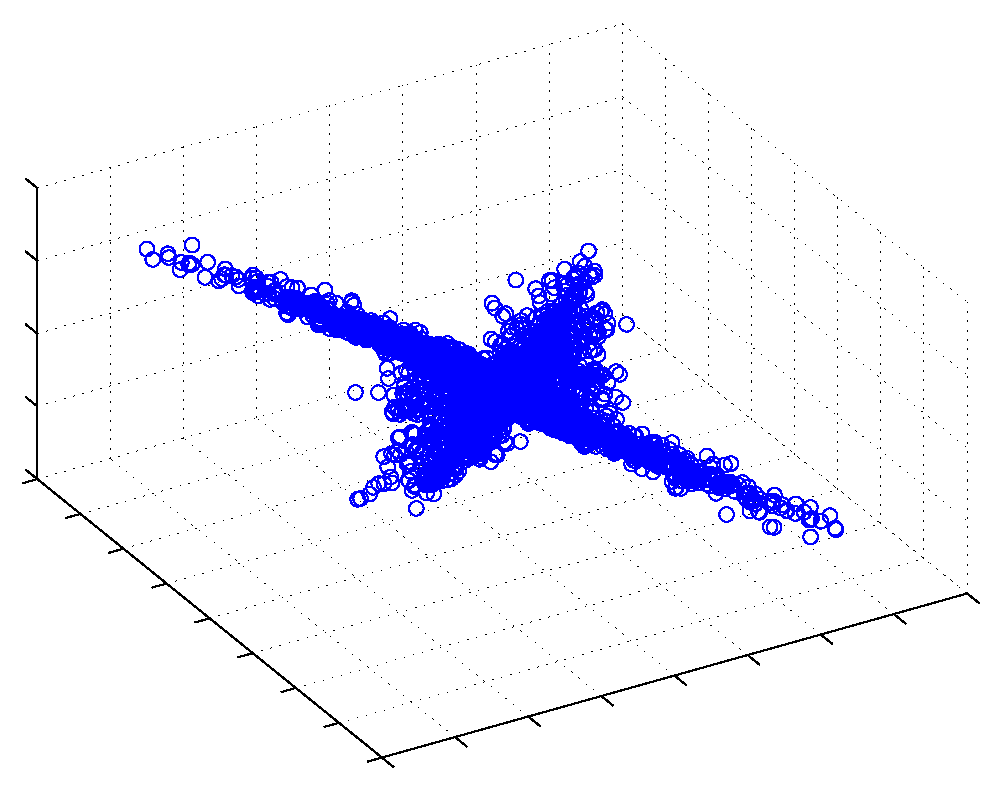
\includegraphics[width=0.45\linewidth]{img/color_components_alex_3d.eps}
  }\quad
\subfigure{
  \includegraphics[width=0.45\linewidth]{img/color_components_matthew_3d.eps} 
  }
}
\label{components}
\caption{Visualization of color components for (left) AlexNet and (right) MattNet.}
\end{figure}


\begin{figure}[t]
\mbox{
  \subfigure{
      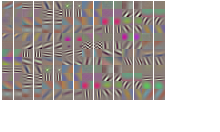
\includegraphics[width=0.45\linewidth]{img/denoising_alex.png}
  }\quad
\subfigure{
  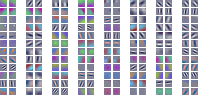
\includegraphics[width=0.45\linewidth]{img/denoising_matthew.png} 
  }
}
\label{denoising}
\caption{Left column depicts original filters, while the right one approximated one with 12 clusters for (left) AlexNet and (right) MattNet (good to look in color). }
\end{figure}


\subsection{Bi-clustering}

